\documentclass{article}
\usepackage{amsfonts}
\usepackage{amsmath}
\usepackage{amssymb}
\usepackage{mathrsfs}
\usepackage{extarrows}
\usepackage{hyperref}
\usepackage[utf8]{inputenc}
\usepackage{graphicx}
\usepackage{mathtools}
\usepackage[a4paper, total={6in, 8in}]{geometry}
\usepackage[table]{xcolor}
\usepackage{tikz}
\usepackage{cancel}
\usetikzlibrary{shapes,arrows, positioning, calc}
\tikzstyle{vertex}=[draw,fill=black!15,circle,minimum size=20pt,inner sep=0pt]
\tikzset{
  treenode/.style = {align=center, inner sep=0pt, text centered,font=\sffamily},
  arn_n/.style = {treenode, rectangle, white, font=\sffamily\bfseries, draw=black,fill=black, minimum width=2.5em,minimum height=1.5em},
  arn_r/.style = {treenode, circle, red, draw=red, minimum width=2.5em, very thick},
  arn_x/.style = {treenode, rectangle, draw=black,minimum width=0.5em, minimum height=0.5em}
}

\newcommand{\accapo}{\\\hspace*{1cm}\\}
\newcommand{\Eaccentata}{$\grave{\text{E}}$ }
\newcommand{\vopen}{``}
\newcommand{\vclose}{''}
\newcommand{\vclosespace}{'' }
\newcommand{\trasformata}{\xrightarrow{\mathscr{F}}}
\newcommand{\antitrasformata}{\xrightarrow{\mathscr{F}^{-1}}}
\newcommand{\intfity}{\int_{-\infty}^{+\infty}}

\setlength{\parindent}{0cm}
% chktex-file 44
% chktex-file 36
% chktex-file 1
\hfuzz=100pt

\title{Orale\\\normalsize fondamenti di telecomunicazioni}
\author{Flavio Colacicchi}
\date{10/01/2024}
\begin{document}
\maketitle
\LARGE\[sorgente\to\boxed{canale}\to destinazione\]\normalsize
più nel dettaglio da parte della sorgente
\[s(t)\to\boxed{ADC}\to s[n]\to\boxed{quantizzatore}\]
La quantizzazione converte il segnale campionato in una sequenza di bit, assegnando ad esempio ai campioni che si trovano nello stesso intervallo di quantizzazione il valor medio tra i due anche se i due campioni differiscono, ad esempio se l'intervallo di quantizzazione per il bit 00 è [0,1] sia 0,3 che 0,7 saranno quantizzati in 00. Questo introduce un errore di quantizzazione che è una variabile aleatoria
\[\left[-\frac{\Delta}{2},\frac{\Delta}{2}\right]\ni e_q[n]=x[n]-x_q[n]\]
Prendendo \(M\) intervalli di campionamento per quantizzare il segnale in elementi da \(K=\log_{2}M\)bit il segnale che ha ampiezza \([-V,V]\) possiamo trovare l'ampiezza di un intervallo di quantizzazione
\[\Delta=\frac{2V}{M}\]
e da qui possiamo vedere che la sua densità di probabilità
\[p_E(e)=\frac{1}{\Delta}rect\left(\frac{e}{\Delta}\right)\]
Ovviamente all'aumentare di \(M\) si riduce \(e_q[n]\) (ad edempio per la radio e la tv si usa \(M=16\)). Si vede facilmente che \(e_q\) è uniformemente distribuita, quindi posso calcolarne la potenza
\[P_e=\frac{1}{\Delta}\int_{-\frac{\Delta}{2}}^\frac{\Delta}{2}e^2de=\frac{e^3}{3\Delta}\Big|_{-\frac{\Delta}{2}}^\frac{\Delta}{2}=\frac{\Delta^2}{12}\]
E da questo ottengo
\[\sigma^2_E=p_E(e)\hspace{2cm}\mu_E=0\]
Riscrivo la potenza in funzione di \(V\) e \(M\)
\[P_e=\frac{\Delta^2}{12}=\frac{4V^2}{12M^2}=\frac{V^2}{3M^2}\]
Se scrivo la potenza in scala logaritmica ottengo
\[{(P_e)}_{dB}=10\log_{10}\frac{V^3}{3}-10\log_{10}M^2=10\log_{10}\frac{V^3}{3}-10\log_{10}2^{2K}\xlongequal{10\log_{10}2=3}10\log_{10}\frac{V^3}{3}-6K\]
Se considero il segnale \(x\) uniformemente distribuito si \([-V,V]\) ottengo la densità di probabilità
\[p_X(x)=\frac{1}{2V}rect\left(\frac{x}{2V}\right)\]
Da qui ottengo la potenza
\[P_x=\frac{1}{2V}\int_{-V}^V x^2dx=\frac{1}{2V}\frac{x^3}{3}\Bigg|_{-V}^V=\frac{V^2}{3}\]
Quindi
\[{(P_e)}_{dB}={(P_x)}_{dB}-6K\]
Se prendiamo la frequenza di campionamento \(f_c=8\text{kHz}\Rightarrow T_c=125\mu\)s e \(K=8\Rightarrow 64\)kb/s abbiamo la pulse code modulation, che è la base della trasmissione dei segnali. Dato che la banda è una risorsa preziosa si fa una codifica di sorgente.\\
Un esempio è la codifica naturale dove si associa alsibolo con valore più basso la parola con tutti 0 e a quello più alto quella con tutti 1 ma non è la più efficiente dato che alcune parole di codice potrebbero non essere usate mai, quindi spesso si usa una codifica fatta appositamente per il tipo di segnale in cui si associano ai simboli più comuni parole con meno bit e a quelli più rari quelle con più bit, risparmiando così banda usando simboli con numero di bit variabile che riduce il numero medio di bit usati.\\
Esempio
Prese le probabilità dei simboli
\[[0.02,0.29,0.03,0.04,0.33,0.04,0.06,0.19]\]
costruiamo un albero (di Huffman) mettendo prima nelle foglie i due valori minori, in questo caso 002 e 003 e mettendo come loro genitore la loro somma, 005 che è molto simile ai valori 004 ripetuto due volte e 006, le metto come foglie mettendo in ordine cresscente da destra verso sinistra e ripetendo la procedura precedente, sommando quindi i due 004 e lo 005 con 006, ottenendo rispettivamente 008 e 011 che non sono confrontabili con gli altri bit, quindi li sommo tra di loro ottenendo 019 che è confrontabile con 019, 029 e 033, così ho preso tutti i bit, ora ripeto la procedura fino a ottenere la radice che dovrebbe venire 1.
\begin{center}
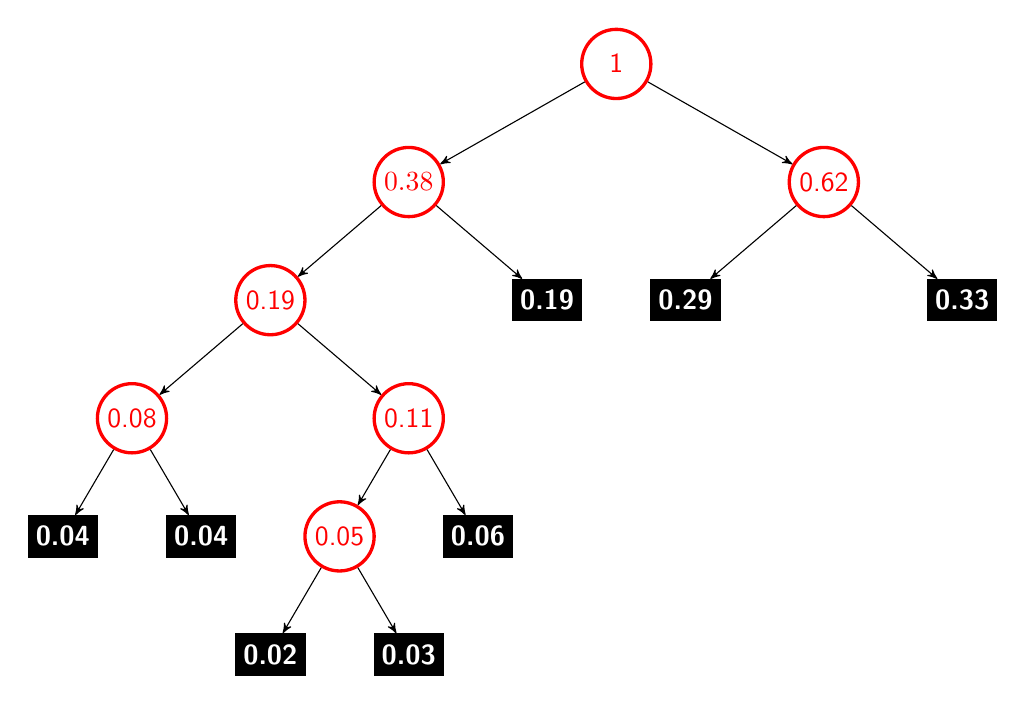
\begin{tikzpicture}[->,>=stealth',level 1/.style={sibling distance=15em},
    level 2/.style={sibling distance=10em},
    level 3/.style={sibling distance=10em},
    level 4/.style={sibling distance=5em}] 
  \node [arn_r] {1}
      child{ node [arn_r] {$0.38$} 
              child{ node [arn_r] {0.19} 
                child{ node [arn_r] {0.08}
                child{ node [arn_n] {0.04}}
                child{node [arn_n] {0.04}}
                }
                child{ node [arn_r] {0.11}
                child{node [arn_r] {0.05}
                    child{node [arn_n] {0.02}}
                    child{node [arn_n] {0.03}}
                }
                child{node [arn_n] {0.06}}
                }
              }
              child{ node [arn_n] {0.19}}                            
      }
      child{ node [arn_r] {0.62}
              child{ node [arn_n] {0.29}}
              child{ node [arn_n] {0.33}}
          }
  ; 
  \end{tikzpicture}
\end{center}
Con questo albero possiamo distribuire i bit di codifica aggiungendo a ogni figlio sinitro 1 alla codifica e a ogni fliglio destro 0. Così facendo ottengo la seguente codifica
\begin{center}
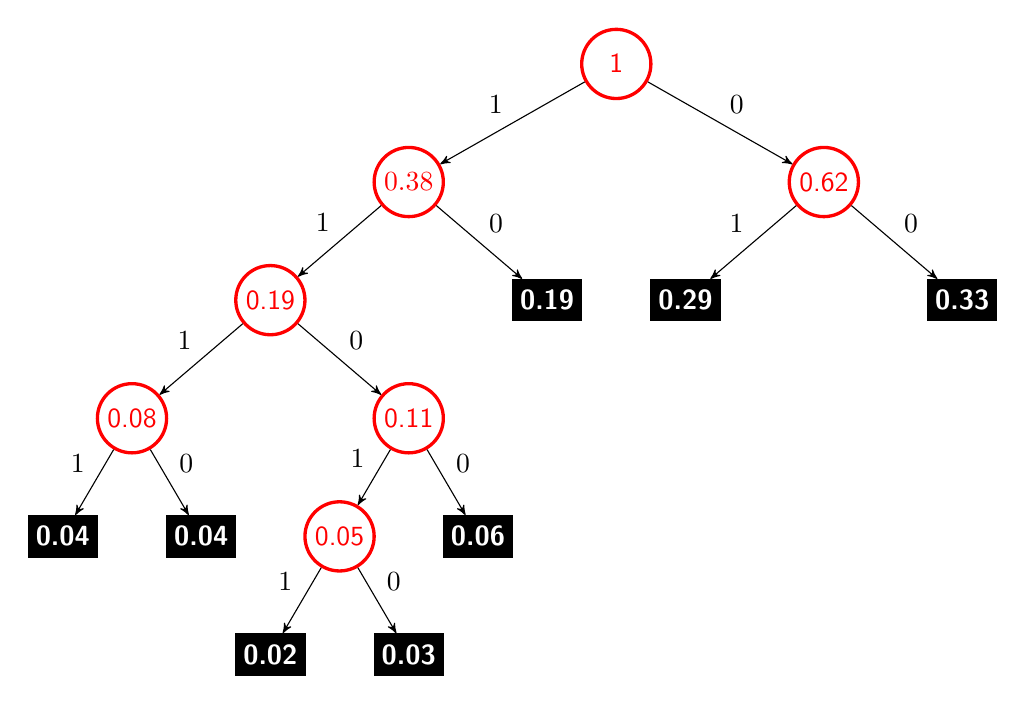
\begin{tikzpicture}[->,>=stealth',level 1/.style={sibling distance=15em},
    level 2/.style={sibling distance=10em},
    level 3/.style={sibling distance=10em},
    level 4/.style={sibling distance=5em}] 
  \node [arn_r] {1}
      child{ node [arn_r] {$0.38$}  
              child{ node [arn_r] {0.19} 
                child{ node [arn_r] {0.08}
                child{ node [arn_n] {0.04} edge from parent node[above left]{$1$}}
                child{ node [arn_n] {0.04}edge from parent node[above right]{$0$}}
                edge from parent node[above left]{$1$}  
                }
                child{ node [arn_r] {0.11}
                child{node [arn_r] {0.05}
                    child{node [arn_n] {0.02} edge from parent node[above left]{$1$}  }
                    child{node [arn_n] {0.03}edge from parent node[above right]{$0$}}
                    edge from parent node[above left]{$1$}  
                }
                child{node [arn_n] {0.06}edge from parent node[above right]{$0$}}
                edge from parent node[above right]{$0$}
                }
                edge from parent node[above left]{$1$}  
              }
              child{ node [arn_n] {0.19}edge from parent node[above right]{$0$}}
              edge from parent node[above left]{$1$}                         
      }
      child{ node [arn_r] {0.62}
              child{ node [arn_n] {0.29} edge from parent node[above left]{$1$}}
              child{ node [arn_n] {0.33}edge from parent node[above right]{$0$}}
              edge from parent node[above right]{$0$}
          }
  ; 
  \end{tikzpicture}
\end{center}
\[\begin{matrix}
    0.19&10\\
    0.29&01\\
    0.33&00\\
    0.04&1111\\
    0.04&1110\\
    0.06&1100\\
    0.02&11011\\
    0.03&11010
\end{matrix}\]
La ripetizione degli 0.04 è dovuto al fatto che due simboli hanno la setssa probabilità. Il numero medio di bit usati è quindi
\[\#bit=\sum_{i=1}^M p_i K_i=0.33\cdot 2+0.23\cdot 2+\cdots=2.43\text{kb/s}<3\text{ che sarebbero quelli usati dalla codifica naturale}\]
E questo sistema garantisce la leggibilità de segnale dato che nessuna parole è inizio di un'altra.\accapo\hspace*{1cm}\accapo
\Eaccentata possibile usare un quantozzatore a intervalli non costanti, ad esempio
\[V_1\to\Delta_1=8\hspace{1cm}V_2\to\Delta_2=4\hspace{1cm}V_3\to\Delta_3=2\hspace{1cm}V_4\to\Delta_4=2\]
quindi
\[p_1=0.5\hspace{1cm}p_2=0.25\hspace{1cm}p_3=p_4=0.125\]
Per calcolare la potenza dell'errore di quantizzazione considero tutti gli intervalli coma variabili aleatorie indipendenti e ottengo
\[P_e=\frac{{\Delta_1}^2}{12}p_1+\frac{{\Delta_2}^2}{12}p_2+\frac{{\Delta_3}^2}{12}p_3+\frac{{\Delta_4}^2}{12}p_4=\frac{37}{12}\]
In codifica naturale mi servirebbero 2 bit per simbolo ma noi vogliamo ottimizzare quindi creiamo ora l'albero di Huffman e ottengo la codifica
\[\begin{matrix}
    V_1&0\\
    V_2&10\\
    V_3&110\\
    V_3&111\\
\end{matrix}\]
Quindi
\[\#bit=0.5\cdot 1+0.25\cdot 2+0.125\cdot 3+0.125\cdot 3=1.75=\frac{7}{4}<2\]
Ma qual'è il numero minimo di bit che posso usare per trasmettere un segnale senza perdere l'informazione? questo numero è l'entropia della sorgente
\[H=\sum_{i=1}^M p_i\log_{2}\frac{1}{p_1}=-\sum_{i=1}^M p_i\log_2 p_i\]
Che in alcuni casi è ottenibile ma non esiste un modo univoco per ottenerlo, dipende dai casi. Si chiama informazione
\[I=\log_2\frac{1}{p_i}\]
La quantità di informazione contenuta in un simbolo. Quindi l'entropia della sorgente è
\[H=\sum_{i=1}^M p_i I_i\]
Quindi se un simbolo ha \(p_i=1\Rightarrow H=0\) mentre se tutti i simboli sono equiprobabili \(p_i=\frac{1}{M}\Rightarrow H=\sum_{i=1}^M\frac{1}{M}\log_2 M=\log_2 M\). Se \(M=2\Rightarrow H=p\log_2\frac{1}{p}+(1-p)\log_2\frac{1}{1-p}\)
\newpage
\Huge
\begin{center}Codifica di linea\end{center}
\large
\[S\to\boxed{\text{sorgente}}\to\boxed{\text{canale}}\to{\text{modulatore}}\to\boxed{\text{trasmettitore}}\to\boxed{canale}\xleftarrow{+}n(t)\to\]
\[\to\boxed{\text{ricevitore}}\to\boxed{\text{filtro}}\to\text{demodulazione}\to\boxed{\text{canale}}\to\boxed{\text{sorgente}}\to D\]\normalsize
La codifica di linea aggiunge bit per correggere l'errore dovuto al rumore, l'esempio supra riportato è una codifica di linea di modulazione. Tutti i canali attenuano le frequenze alte quindi i canali possono essere visti come dei filtri passsa basso con banda pari alla frequenza massima che lasciano passare, inoltr eviene introdotto del rumore (che vediamo ocme un rumore bianco gaussiano). Nella modulazione moltipico il segnale per una frequenza portante. Dopo che il segnale viene ricevuto dal ricevitore si passa per un filtro, solitamente basato sualla frequenza portante (I segnali wireless sono modellati con delle rect cejtrate in \(\pm f_0\) e di ampiezza \(B\) che è la banda) per ridurre la potenza del rumore prima della demodulazione che contiene
\[\to\boxed{\text{D.A.C}}\to\boxed{\text{decisore a soglia}}\to\]
Dove il decisore a soglia è un sistema di confronto che confronta il segnale ricevuto con una soglia per vedere se il valore ricevuto è uno 0 o un 1. Una cosa fondamentale nella trasmissione del segnale è il \textbf{diagramma ad occhio} che stabilisce una zona in cui il segnale non deve entrare altrimenti diventa non legggibile da decisore a soglia. Le codifiche possono essere del tipo \vopen return to 0\vclose, dove il segbale torna a 0 prima di trasmettere il bit successivo, in questo caso il diagramma ad occhio è così
\begin{center}
    \includegraphics[height=4.5cm]{images/eye diagram-2.png}
\end{center}
Mentre se si usa una modulazione che non torna a 0 prima di trasmettere il diagramma ad occhio simile a questa
\begin{center}
    \includegraphics[height=4.5cm]{images/eye diagram.png}
\end{center}
Per velocizzare le trasmissioni si tende a non usare una trasmissione binaria ma una trasmissione M-aria, ovvero con M simboli, ad esempio per il wifi si usano 256 simboli
\accapo
Un esempio: sia il nostro alfabeto
\[c_m\in\{c_1,c_2,\dots,c_M\}\]
e il tempo di trasmissione di un simbolo
\[T_s\]
e quindi il baudrate è
\[R_s=\frac{1}{T_s}\]
quindi il bitrate di trasmissione, che è il tempo per ogni simbolo moltiplicato per il bit di ogni simbolo, si calcola
\[R_b=R_s\log_{2}M\]
Ora prendiamo
\[M=4\hspace{2cm} c_m=\{-1,-0.5,0.5,1\}\]
E vogliamo trasmettere la sequenza
\[s[n]=[1,0.5,-0.5,1]\]
Ora lo moduliamo e otteniamo un'onda da trasmettere
\[x(t)=\sum_{n=1}^{length(s[n])}s[n]g(t-nT_s)\]
Dove \(g(t)\) è l'impulso base che deve essere
\[g(t)=\begin{cases}
    1&t=0\\
    0&t=kT_s,k\in\mathbb{Z}\setminus\{0\}
\end{cases}\]
E si cerca di rimanere nel caso in cui la sua trasformata resta limitata in banda per evitare di usarne troppa in quanto è una risorsa preziosa. Quindi un segnale tipicamente usato è
\[g(t)=sinc\left(\frac{t}{T_s}\right)\]
Dato che la sua trasformata
\[G(f)=rect(T_s f)\]
\Eaccentata quindi limitata in banda. Un altro impulso molto usato è quello di Nyquist a coseno rialzato (\(\beta\) nel grafico è il rolloff)
\begin{center}
    \includegraphics[width=8cm]{images/impulso di nyquist.png}
\end{center}
Facciamo un altro esempio di trasmissione con un segnale binario
\[s[n]\in\{c_1,c_2\}\]
\[x(t)=\sum_{n=-\infty}^{+\infty}s[n]g(t-nT_s)\]
Ora dobbiamo aggiungere il rumore e il passaggio per il canale
\[y(t)=x(t)*h(t)+n(t)=x(t)+n(t)\]
quindi il nostro segnale non verrà fuori pulito ma a causa del rumore diventa \vopen frastagliato\vclose\space
\begin{center}
    \includegraphics[width=10cm]{images/eye diagram noise.jpg}
\end{center}
Considerando che il rumore ha una densità di probabilità gaussiana possiamo vedere \(y(t)\) come una variabile aleatoria
\[Y=y(0)=x+n=\begin{cases}
    c_1+n\\
    c_2+n
\end{cases}\]
\[P_N(n)=\frac{1}{\sqrt{2\pi}\sigma_n}e^{-\frac{n^2}{2{\sigma^2}_n}}\hspace{2cm}{\sigma^2}_n=BN_0\]
\[P_Y(y)=\frac{1}{\sqrt{2\pi}\sigma_n}e^{-\frac{-{(y-c_i)}^2}{2{\sigma^2}_n}}\]
\[p_r\{y<\overline{c}|c_2\}=\int_{-\infty}^{\overline{c}}R_Y(y)dy=\int_{-\infty}^{\overline{c}}\frac{1}{\sqrt{2\pi}\sigma_n}e^{-\frac{-{(y-c_2)}^2}{2{\sigma^2}_n}}dy\xlongequal{t=\frac{c_2-y}{\sqrt{2}\sigma_n}}=\int_{+\infty}^{\frac{c_2-\overline{c}}{\sqrt{2}\sigma_n}}\frac{1}{\sqrt{2\pi}\sigma_n}e^{-t^2}(-dt\sqrt{2}\sigma_n)=\]
\[=\int_{\frac{c_2-\overline{c}}{\sqrt{2}\sigma_n}}^{+\infty}\frac{1}{\sqrt{\pi}}e^{-t^2}=\frac{1}{2}erfc\left(\frac{c_2-\overline{c}}{\sqrt{2}\sigma_n}\right)=Q\left(\frac{c_2-\overline{c}}{\sigma_n}\right)\]
\[p_r\{y>\overline{c}|c_1\}=\int_{\overline{c}}^{+\infty}e^{-\frac{{{(y-c_1)}^2}}{2{\sigma^2}_n}}\frac{1}{\sqrt{2\pi}\sigma_n}dy=\frac{1}{2}erfc\left(\frac{\overline{c}-c_1}{\sqrt{2}\sigma_n}\right)=Q\left(\frac{\overline{c}-c_1}{\sigma_n}\right)\]
Se oglio calcolare il bit error rate (BER) devo fare la sommatoria delle probabilità di ciascun simbolo per la rispettiva \(Q\), quindi in questo caso
\[BER=\frac{1}{2}Q\left(\frac{\overline{c}-c_1}{\sigma_n}\right)+\frac{1}{2}Q\left(\frac{c_2-\overline{c}}{\sigma_n}\right)\]
che in questo caso è
\[BER=Q\left(\frac{c_2-c_1}{\sigma_n}\right)=Q\left(\frac{d}{\sigma_n}\right)=Q\left(\frac{d}{\sqrt{N_0 B}}\right)\]
\end{document}